\subsection{Problematiza\c c\~ao da Revis\~ao} \label{subsec: problematização da revisão}

Nesta seção é abordado um problema de pesquisa que pode ser compreendido por vários leitores na Figura \ref{fig:serie-temporal} é apresentado um mapa conceitual de publicação e os autores são o pilar mais relevante para a revisão porque apresentam vários modelos que servirão de base e como se trata de séries temporais a previsão que pode ser feita neste contexto é um problema de grande significado em si mesmo.

\begin{figure}[H]
	\centering
	\caption{Mapa conceitual do problema de pesquisa}
	\label{fig:serie-temporal}
	\includegraphics[width=0.9\linewidth]{Revisao/Figuras/"Série temporal"}
	
	Fonte: Elaboração própria 
\end{figure}

No mapa conceitual apresentado na Figura \ref{fig:serie-temporal} é visto o problema sendo relacionado com palavras, tornando evidente o que será abordado durante o trabalho, deixando as questões de pesquisa em tópicos logo à frente.

\begin{enumerate}[start=1, label = {\textbf{Q} \arabic* } ]
	\item \label{questão:rev1}Quais os autores que mais publicam sobre o assunto de séries temporais?
	\item \label{questão:rev2}Quais os países que mais publicam sobre o assunto? 
	\item \label{questão:rev3}Quais as áreas que mais publicam sobre o tema?
	\item \label{questão:rev4}Quais são as obras mais influentes na análise de séries temporais?
\end{enumerate}

\subsection{Metodologia}\label{subsec:met da revisão}

Nesta seção é esclarecido como a revisão foi conduzida desde a análise do banco de dados até a conclusão da revisão.

\begin{figure}[H]
	\centering
	\caption{Etapas da Revisão.}
	\label{fig:rsl}
	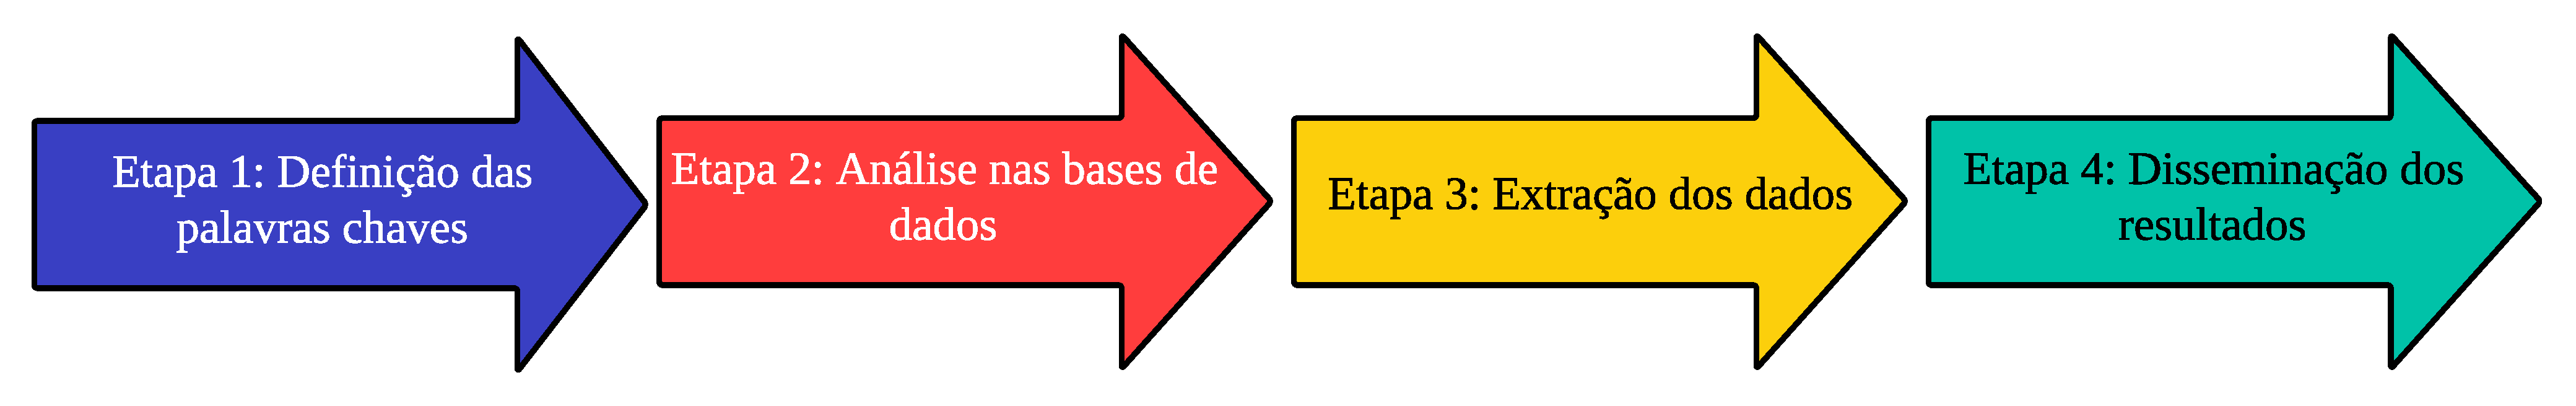
\includegraphics[width=0.9\linewidth]{Revisao/Figuras/RSL}
	
	Fonte: Adaptado de \citeonline{MARTINS201671}
\end{figure}
\begin{enumerate}[start=1, label = {\textbf{Etapa} \arabic* } ]
	
	
	\item \label{etp:rev-1}A Figura \ref{fig:rsl} usa uma adaptação de \citeonline{MARTINS201671} para esta revisão sistemática que está sendo analisada. Depois, há as buscas nos bancos de dados Scopus, Web of Science e Lens. No início foram utilizadas algumas bases no meio de tantas na literatura para melhor atender ao tema da pesquisa.
	
	
\textbf{Campo de pesquisa Scopus}

\textbf{\textit{TITLE-ABS-KEY (``time series forecasting")  AND  TITLE-ABS-KEY (``time series analysis")  AND  ( LIMIT-TO ( DOCTYPE ,  ``ar" ) )  AND  ( LIMIT-TO ( LANGUAGE ,  ``English" ) )  AND  ( LIMIT-TO ( PUBYEAR ,  2022 )  OR LIMIT-TO ( PUBYEAR ,  2021 )  OR  LIMIT-TO ( PUBYEAR ,  2020 )  OR  LIMIT-TO ( PUBYEAR ,  2019 )  OR  LIMIT-TO ( PUBYEAR ,  2018 )  OR  LIMIT-TO ( PUBYEAR ,  2017 ) )}}

\textbf{Campo de pesquisa na Web of Science}

\textit{\textbf{``times series forecasting" (All Fields) and ``time series analysis" (All Fields)}} (Publication Years: 2022 or 2021 or 2020 or 2019 or 2018 or 2017) (Document Types: Articles) (Languages: English)

\textbf{Campo de pesquisa de Lens}

\textit{\textbf{Scholarly Works (11) = ( ``time series forecasting" ) AND ( ( ``time series analysis" ) AND ( ``nonlinear forecasting" ) ) }}
Filters: Year Published = ( 2016 - 2022  ) Publication Type = ( journal article  )\\
	
	Em todos os campos de busca, foram utilizados os últimos 6 anos, com exceção do site do Lens, onde optamos por 6 anos porque ele devolvia poucos artigos. Nesta etapa, usamos as palavras-chave que melhor se adaptam à busca \textit{time series forecasting and time series analysis and nonlinear forecasting}.
	
	
	\item \label{etp:rev-2} No cruzamento de palavras obtém-se um número considerável de artigos sem restringir a área em que cada artigo pode ser publicado. Na Tabela \ref{tb1} foi feita uma tabulação dos resultados obtidos sem excluir a duplicata que trataremos na seção \ref{subesec:resul da revisão}.
	
	\item \label{etp:rev-3}Esta etapa é avaliar cada dado obtido sem nenhum filtro no início da busca, a extração destes dados sem utilizar nenhum filtro anual nas buscas seria muitos artigos para analisar, por exemplo, no banco de dados Scopus seria com artigos de $498$, na Web of Sceince seria com artigos de $140$, e na Lente como não retorna muitos artigos é com $11$ dando um total de $649$ sem remover duplicata. É correto lembrar que estes artigos têm apenas o filtro da língua inglesa e do artigo, para melhorar a busca e a tomada de decisão usando o filtro dos anos, os últimos 6 anos é um valor mais agradável de artigos para usar com pouco tempo para analisar, e usando a diferença entre esta estimativa que foi feita na Tabela \ref{tb1} são menos de $356$ artigos para analisar. Lembrando que se a remoção de duplicatas foi feita, este número que foi obtido no resultado de todas as bases pode atingir um número ainda menor do que o pretendido neste trabalho.
	
	\item  \label{etp:rev-4}Nesta etapa é mais analisar a dimensão do que está sendo trabalhado, fazendo a análise das áreas e lendo os artigos que são realmente importantes para a revisão. Como esta revisão está focada em séries temporais em um programa mestre de engenharia de produção e sistemas, vale a pena analisar a correlação. Desta forma, uma das áreas é a matemática, por isso foi selecionada nestes artigos que uma análise mais profunda dos artigos das séries temporais pode resultar se olharmos as áreas de especialização dos artigos pesquisados, como pode ser visto na Figura \ref{fig:areas} que as áreas aqui citadas com grande relevância são \textbf{informática, engenharia e matemática} tem um número muito alto de publicações representando $50\%$ da pesquisa, então a pesquisa está no caminho certo usando matemática básica para ter uma estimativa de quantos artigos podem ser eliminados seria cerca de $481$ artigos, mas isto sem muita base que este número tem uma precisão. Usando o \textit{software mendeley desktop} para estipular o valor exato de quantos artigos podem ser usados sem duplicação é deixado com um número de artigos de $308$.
\end{enumerate}